% Template for PLoS
% Version 3.4 January 2017
%
% % % % % % % % % % % % % % % % % % % % % %
%
% -- IMPORTANT NOTE
%
% This template contains comments intended 
% to minimize problems and delays during our production 
% process. Please follow the template instructions
% whenever possible.
%
%
% -- FIGURES AND TABLES
%
% Please include tables/figure captions directly after the paragraph where they are first cited in the text.
%
% DO NOT INCLUDE GRAPHICS IN YOUR MANUSCRIPT
% - Figures should be uploaded separately from your manuscript file. 
% - Figures generated using LaTeX should be extracted and removed from the PDF before submission. 
% - Figures containing multiple panels/subfigures must be combined into one image file before submission.
% For figure citations, please use "Fig" instead of "Figure".
% See http://journals.plos.org/plosone/s/figures for PLOS figure guidelines.
%
% Tables should be cell-based and may not contain:
% - spacing/line breaks within cells to alter layout or alignment
% - do not nest tabular environments (no tabular environments within tabular environments)
% - no graphics or colored text (cell background color/shading OK)
% See http://journals.plos.org/plosone/s/tables for table guidelines.
%
% For tables that exceed the width of the text column, use the adjustwidth environment as illustrated in the example table in text below.
%
% % % % % % % % % % % % % % % % % % % % % % % %
%
% -- EQUATIONS, MATH SYMBOLS, SUBSCRIPTS, AND SUPERSCRIPTS
%
% IMPORTANT
% Below are a few tips to help format your equations and other special characters according to our specifications. For more tips to help reduce the possibility of formatting errors during conversion, please see our LaTeX guidelines at http://journals.plos.org/plosone/s/latex
%
% For inline equations, please be sure to include all portions of an equation in the math environment.  For example, x$^2$ is incorrect; this should be formatted as $x^2$ (or $\mathrm{x}^2$ if the romanized font is desired).
%
% Do not include text that is not math in the math environment. For example, CO2 should be written as CO\textsubscript{2} instead of CO$_2$.
%
% Please add line breaks to long display equations when possible in order to fit size of the column. 
%
% For inline equations, please do not include punctuation (commas, etc) within the math environment unless this is part of the equation.
%
% When adding superscript or subscripts outside of brackets/braces, please group using {}.  For example, change "[U(D,E,\gamma)]^2" to "{[U(D,E,\gamma)]}^2". 
%
% Do not use \cal for caligraphic font.  Instead, use \mathcal{}
%
% % % % % % % % % % % % % % % % % % % % % % % % 
%
% Please contact latex@plos.org with any questions.
%
% % % % % % % % % % % % % % % % % % % % % % % %

\documentclass[10pt,letterpaper]{article}
\usepackage[top=0.85in,left=2.75in,footskip=0.75in]{geometry}

% amsmath and amssymb packages, useful for mathematical formulas and symbols
\usepackage{amsmath,amssymb}

% Use adjustwidth environment to exceed column width (see example table in text)
\usepackage{changepage}

% Use Unicode characters when possible
\usepackage[utf8x]{inputenc}

% textcomp package and marvosym package for additional characters
\usepackage{textcomp,marvosym}

% cite package, to clean up citations in the main text. Do not remove.
\usepackage{cite}

% Use nameref to cite supporting information files (see Supporting Information section for more info)
\usepackage{nameref,hyperref}

% line numbers
\usepackage[right]{lineno}

% ligatures disabled
\usepackage{microtype}
\DisableLigatures[f]{encoding = *, family = * }

% color can be used to apply background shading to table cells only
\usepackage[table]{xcolor}

% array package and thick rules for tables
\usepackage{array}

% create "+" rule type for thick vertical lines
\newcolumntype{+}{!{\vrule width 2pt}}

% create \thickcline for thick horizontal lines of variable length
\newlength\savedwidth
\newcommand\thickcline[1]{%
	\noalign{\global\savedwidth\arrayrulewidth\global\arrayrulewidth 2pt}%
	\cline{#1}%
	\noalign{\vskip\arrayrulewidth}%
	\noalign{\global\arrayrulewidth\savedwidth}%
}

% \thickhline command for thick horizontal lines that span the table
\newcommand\thickhline{\noalign{\global\savedwidth\arrayrulewidth\global\arrayrulewidth 2pt}%
	\hline
	\noalign{\global\arrayrulewidth\savedwidth}}


% Remove comment for double spacing
%\usepackage{setspace} 
%\doublespacing

% Text layout
\raggedright
\setlength{\parindent}{0.5cm}
\textwidth 5.25in 
\textheight 8.75in

% Bold the 'Figure #' in the caption and separate it from the title/caption with a period
% Captions will be left justified
\usepackage[aboveskip=1pt,labelfont=bf,labelsep=period,justification=raggedright,singlelinecheck=off]{caption}
\renewcommand{\figurename}{Fig}

% Use the PLoS provided BiBTeX style
\bibliographystyle{plos2015}

% Remove brackets from numbering in List of References
\makeatletter
\renewcommand{\@biblabel}[1]{\quad#1.}
\makeatother

% Leave date blank
\date{}

% Images
\usepackage{graphics}
\graphicspath{ {img/} }

% Header and Footer with logo
\usepackage{lastpage,fancyhdr,graphicx}
\usepackage{epstopdf}
\pagestyle{myheadings}
\pagestyle{fancy}
\fancyhf{}
\setlength{\headheight}{27.023pt}
%\lhead{
\includegraphics[width=2.0in]{PLOS-submission.eps}}
\rfoot{\thepage/\pageref{LastPage}}
\renewcommand{\footrule}{\hrule height 2pt \vspace{2mm}}
\fancyheadoffset[L]{2.25in}
\fancyfootoffset[L]{2.25in}
\lfoot{\sf KTH}

% Custom includes
\usepackage[normalem]{ulem}
\useunder{\uline}{\ul}{}
\usepackage{booktabs}
%% Include all macros below
\DeclareMathOperator*{\argmin}{arg\,min}
\DeclareMathOperator*{\argmax}{arg\,max}
%% END MACROS SECTION


\begin{document}
	\vspace*{0.2in}
	
	% Title must be 250 characters or less.
	\begin{flushleft}
		{\Large
			\textbf\newline{Predicting signal peptides using machine learning} % Please use "sentence case" for title and headings (capitalize only the first word in a title (or heading), the first word in a subtitle (or subheading), and any proper nouns).
		}
		\newline
		% Insert author names, affiliations and corresponding author email (do not include titles, positions, or degrees).
		\\
		Jonas Andersson
		\\
		\bigskip
		Computer Science and Communications, KTH Royal Institute of Technology, Stockholm, Sweden
		\bigskip
		
		% Insert additional author notes using the symbols described below. Insert symbol callouts after author names as necessary.
		% 
		% Remove or comment out the author notes below if they aren't used.
		%
		% Primary Equal Contribution Note
		%\Yinyang These authors contributed equally to this work.
		
		% Additional Equal Contribution Note
		% Also use this double-dagger symbol for special authorship notes, such as senior authorship.
		%\ddag These authors also contributed equally to this work.
		
		% Current address notes
		%\textcurrency Current Address: Dept/Program/Center, Institution Name, City, State, Country % change symbol to "\textcurrency a" if more than one current address note
		% \textcurrency b Insert second current address 
		% \textcurrency c Insert third current address
		
		% Deceased author note
		%\dag Deceased
		
		% Group/Consortium Author Note
		%\textpilcrow Membership list can be found in the Acknowledgments section.
		
		% Use the asterisk to denote corresponding authorship and provide email address in note below.
		* jonand8@kth.se
		
	\end{flushleft}
	% Please keep the abstract below 300 words
	\section*{Abstract}
	We test three different classifiers against a test set of data to shed light on what techniques makes a good classifier. The classifiers are then used on two proteomes to infer signal peptide sequences. The classification pipeline combines N-gram language modeling with a vector space model using TF-IDF term weighting to provide data abstraction along with knowledge of the signal peptide structure to boost prediction accuracy on the test set of data. 
	
	
	% Please keep the Author Summary between 150 and 200 words
	% Use first person. PLOS ONE authors please skip this step. 
	% Author Summary not valid for PLOS ONE submissions.   
	%\section*{Author summary}
	%Lorem ipsum dolor sit amet, consectetur adipiscing elit. Curabitur eget %porta erat. Morbi consectetur est vel gravida pretium. Suspendisse ut dui %eu ante cursus gravida non sed sem. Nullam sapien tellus, commodo id velit %id, eleifend volutpat quam. Phasellus mauris velit, dapibus finibus %elementum vel, pulvinar non tellus. Nunc pellentesque pretium diam, quis %maximus dolor faucibus id. Nunc convallis sodales ante, ut ullamcorper est %egestas vitae. Nam sit amet enim ultrices, ultrices elit pulvinar, %volutpat risus.
	
	\linenumbers
	
	% Use "Eq" instead of "Equation" for equation citations.
	\section*{Introduction}
	The localization of proteins is mostly determined by a biological trafficking system. When proteins are synthesized on cytoplasmic ribosomes and have several possible destinations such as the nuclear, mitochondria, or peroxisomes. Signal peptides direct proteins to their proper destination after synthesis, keeping them from arriving at the wrong cellular location. Signal peptides, short chains of amino acids, act as postal codes for their destination. These sorting signals, a N-terminal signal peptide, are removed or cleaved off. If the protein does not have this signal peptide then it remains in the cytoplasm. The structure of the signal peptide consists of a positively charged N-region (1-5 residues long), a hydrophobic h-region (7-15 residues long), and finally a polar C-region (3-7 residues long). The cleavage point is in the C-region, but the location varies between proteins \cite{thesis}. 
	
	There exist a number of computational methods for predicting these sorting signals using distinctly different approaches. It is useful to locate these signals as it can potentially add insight into protein translocation, how chromosomes are rearranged. Some examples of application domains for signal prediction include drug discovery and gene therapy \cite{thesis}. Numbering among these computational approaches are neural networks(NNs), support vector machines(SVMs), hidden markov models (HMMs), decision trees, and ensemble learning methods. These algorithms are encompassed in field of computer science called machine learning. Machine learning (ML) algorithms learn and make decisions from data \cite{wikipedia}. ML comprises a broad spectrum of approaches; much of the work done on signal prediction is approached as a classification problem. In classification, a probability distribution is drawn over the classes, and we choose the class that has the highest probability \cite{jurafsky}. $$ \hat{c} = \argmax_{c \in C}{ \Pr(c \vert x)} $$
	
	\section*{Materials and methods}
	\subsection*{Data Preprocessing}
	The training data is FASTA-like with each sequence followed by an annotation line.  The annotation line marks the location of the n-, h-, and c- regions. The annotation line is removed during preprocessing. The training data is a corpus
	
	\subsection*{Data Modeling}
	The training data is represented using a language model called N-grams. N-gram models are a probabilistic language model which predict the next word or symbol from the previous N-1 words or symbols. Since we are using amino acid residues in place of words, this will instead predict the next residue from the previous N-1 residues. 

	N-gram models are trained on a corpus which is a computer readable collection of text or speech\cite{jurafsky}. The training data is a corpus which contains 2654 examples. The sequence lengths in the corpus range from 16 residues to 4563 residues. With most sequences having a length between 16 and 1000 residues in length as seen in figure \ref{fig:sequence-hist}. 
	
	% For figure citations, please use "Fig" instead of "Figure".
	% Place figure captions after the first paragraph in which they are cited.
	\begin{figure}[!h]
		\centering
		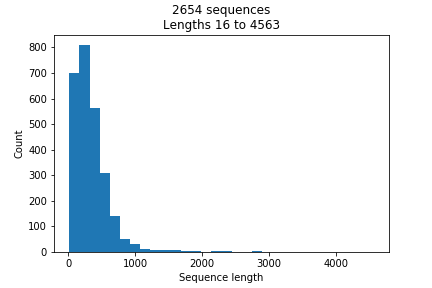
\includegraphics[scale=0.5, width=\textwidth]{sequence-hist}
		\caption{{\bf Training Data Length Histogram}}
		\label{fig:sequence-hist}
	\end{figure}
	
	Once the data is counted, it is vectorized into a vector space model where the sequences are converted into vectors of features representing the amino acids that appear in a sequence. The value of each feature is the term weight and is a function of the terms frequency in the sequence.
	
	The collection of sequences characterized as vectors can be viewed as a sparse matrix of weights where $w_{i,j}$ is the weight of the residue N-gram $i$ in sequence $j$. This matrix is called a term-by-document matrix \cite{jurafsky}.  
	
	The term weighting is not only a function of the frequency but also its inverse frequency. The inverse document frequency, IDF, term weight assigns higher weights to more discriminative terms. Discriminative terms occur in only a few of the sequences. 
	$$ idf_i = \log {\frac{N}{n_i}}$$ We combine IDF with term frequency, TF, to obtain tf-idf weighting. $$w_{i,j} = tf_{i,j} \times idf_i$$ TF-IDF prefers words that are frequent in the current sequence but rare overall in the collection \cite{jurafsky}.
	
	\subsection*{Training and Test Sets}
	The probabilities of the N-gram model come from the corpus it is trained on. The parameters of a statistical model are trained on a set of data and then the model is applied to new unseen data to determine performance. The unseen data set is often called a test set. Using this method we can also evaluate model parameters, such as different orders of N in an N-gram model. Ideally, a models training set should be as large as possible without making the test set unrepresentative. In practice this is typically $80\%$ training, $10\%$ development, and $10\%$ test \cite{jurafsky}. This project does not use a development set so the division will be $80\%$ training and $20\%$ test. 
	
	\subsection*{Classifiers}
	\subsubsection*{Naive Bayes}
	In general, a classifier can be said to be a function that finds the class $C_k$ that is most probable given the observed data:
	
	\begin{equation}
	p(C_k|x_1, \dots ,x_n)
	\end{equation}
	
	\noindent Using Bayes Theorem, we get
	
	\begin{equation}
	p(C_k|x_1,\dots,x_n) \propto p(C_k) p(x_1,\dots,x_n|C_k)
	\end{equation}
	
	\noindent which can be expanded to the following using the chain rule of conditional probabilities: 
	
	\begin{equation}
	\label{eq:chain}
	p(x_1,\dots,x_n|C_k) = p(x_1|x_2\dots,x_n,C_k) \dots p(x_n|C_k)
	\end{equation}
	
	\noindent The conditional probabilities in equation \ref{eq:chain} can be hard to compute. Naive Bayes makes the assumption that the data are independent of each other given the class. We thus get
	
	\begin{equation}
	p(x_i|x_{i+1}\dots,x_n,C_k) = p(x_i|C_k)
	\end{equation}
	
	\noindent Equation \ref{eq:chain} then simplifies to
	
	\begin{equation}
	\begin{gathered}
	p(x_1,\dots,x_n|C_k) = p(x_1|C_k) \dots p(x_n|C_k) \\
	\Rightarrow \\
	p(C_k|x_1,\dots,x_n) \propto p(C_k) p(x_1|C_k) \dots p(x_n|C_k)
	\end{gathered}
	\end{equation}
	
	\noindent Compressing this, the Naive Bayes classifier finds the most likely class $\hat{y}$,
	
	\begin{equation}
	\hat{y} = \argmax_{k} \, p(C_k) \prod_{i=1}^{n} p(x_i|C_k)    
	\end{equation}
	
	\noindent $p(C_k)$ can be estimated by counting the frequencies of the classes in the training set. Similarly, the conditional probabilities $p(x_i|C_k)$ are the frequencies of each residue n-gram in the different classes. To avoid a product of zero if a residue n-gram has never appeared in a class, one can do \textit{smoothing}, which slightly changes all probabilities to avoid zeros. 
	
	Naive Bayes is often employed as a good baseline method, yielding results that are sufficiently good for practical use \cite{jurafsky}. As a baseline, this classifier is expected to perform the worst, but with at least 70 percent accuracy.
	
	\subsubsection*{Support Vector Machines}
	
	Support Vector Machines are a case of a maximal margin classifier that can draw non-linear decision boundaries. Support vector machines are intended for a binary classification setting, such as the problem posed in this project. SVMs make use of a kernel to transform the input space into a higher dimensional space for the purpose of finding the separating hyperplane with maximum margins. There are a number of different non-linear kernels to use, a popular choice is the radial kernel \cite{yellowbook} which takes the form of 
	\begin{equation}
	\label{rbf}
	K(x_i, x_{i^\prime}) = \exp({-\gamma \sum_{j=1}^{p}({x_{ij}-x_{x^\prime j}})^2})
	\end{equation}
	
	When given an observation that has a large euclidean distance from a training observation then the sum $\sum_{j=1}^{p}({x_{ij}-x_{x^\prime j}})^2$ will be large, but the equation \ref{rbf} will be small. This means that it will not affect the classification of points closer to the training data. Support vector machines are considered one of the best 'out of the box' classifiers \cite{yellowbook}. In this experiment we make use of the radial or RBF kernel. It is hypothesized that this will be the strongest classifier of the 3 chosen. 
	
	\subsubsection*{Random Forests}
	Random Forests are a collection of decision tree's. Decision tree's suffer from high variance, because when the training data is split randomly and fit to a decision tree, the results could be different based on the split \cite{yellowbook}. However with random forests, each time a split is considered, a random sample of $m$ predictors is chosen instead of the full set of predictors $p$. A rule of thumb is that the sample $m \approx \sqrt{p}$ \cite{yellowbook}. Sampling only a subset of the total predictors mitigates the effect of very strong predictors. In a standard tree these strong predictors would be candidates for the top split because they maximize the information gain. 
	
	\subsection*{Stafford Noble's Guidelines}
	The guidelines given in 'A Quick Guide to Organizing Computational Biology Projects' \cite{noble} were adhered to for the most part with some small deviations. The deviations were largely due to time constraints. The spirit of the document was followed.
	
	The project directory structure was adhered to as per Stafford Noble. Source code is in a 'src' folder, the doc folder contains the report, data contains the training and proteome data. The bin folder was excluded in favor of a python driver script using argparse. This could have been easily changed into a 'binary' by adding the file to the workstations PATH and removing the extension, but it was deemed unnecessary for the sake of time. 
	
	A lab notebook was kept in the form of a markdown file. The markdown file is the summary of hand written notes and ipython notebooks as well as general brainstorming. 
	
	Documenting the source code was done with docstrings. This deviated as the project deadline drew near and errors were encountered. Some functions went through several revisions and updating the docstrings in the intermediate state would have been a waste of time. Code was prototyped in an ipython notebook (included in the project source files under the notebooks directory) and then transferred to a python module. The scripts written could be classifed as 'project specific' in the 4 categories defined in Stafford Noble. 
	
	The use of version control was followed nearly to the letter. A .gitignore file was used to ignore generated files such as the temporary files generated by python and LaTeX editors. Data was checked in to version control as a time saving measure. This made it easy to pull and push changes when working on different workstations. Normally a function would be used to pull the data from AWS or some other repository purposed for storing data. For the sake of time, data was checked in. 
	% Results and Discussion can be combined.
	\section*{Results and Discussion}
	
	Improving a model lies in understanding where mistakes are made. In a classifier this is done with a confusion matrix (also called a contingency table). A confusion matrix for a 2-way classification task is a $2 \times 2$ matrix, where cell $x,y$ is the number of times an item with correct classification as $x$ was classified by the model as $y$. 
	% Place tables after the first paragraph in which they are cited.

	\begin{table}[!ht]
		\centering
		\caption{{\bf Confusion matrix for transmembrane data}}
		\label{tab:conf-tm}
		\begin{tabular}{lccllcc}
			\multicolumn{3}{l}{Naive Bayes}                                                & \multicolumn{2}{c}{SVM}                                          & \multicolumn{2}{l}{Random Forest} \\ \hline
			& \multicolumn{1}{l}{\textbf{P}} & \multicolumn{1}{l|}{\textbf{N}} & \multicolumn{1}{c}{\textbf{P}} & \multicolumn{1}{c|}{\textbf{N}} & \textbf{P}      & \textbf{N}      \\ \hline
			\textbf{PP} & 47                             & \multicolumn{1}{c|}{0}          & 47                             & \multicolumn{1}{l|}{0}          & 47              & 0               \\
			\textbf{PN} & 12                             & \multicolumn{1}{c|}{0}          & 8                              & \multicolumn{1}{l|}{4}          & 12              & 0               \\ \hline
		\end{tabular}
	\end{table}

	\begin{table}[!ht]
		\centering
		\caption{{\bf Confusion matrix for non-transmembrane data}}
		\label{tab:conf-non-tm}
		\begin{tabular}{ccccccc}
			\multicolumn{3}{c}{Naive Bayes}                            & \multicolumn{2}{c}{SVM}                      & \multicolumn{2}{c}{Random Forest} \\ \hline
			& \textbf{P} & \multicolumn{1}{c|}{\textbf{N}} & \textbf{P} & \multicolumn{1}{c|}{\textbf{N}} & \textbf{P}      & \textbf{N}      \\ \hline
			\textbf{PP} & 187        & \multicolumn{1}{c|}{31}         & 204        & \multicolumn{1}{c|}{14}         & 186             & 32              \\
			\textbf{PN} & 12         & \multicolumn{1}{c|}{243}        & 23         & \multicolumn{1}{c|}{232}        & 42              & 213             \\ \hline
		\end{tabular}
	\end{table}

\begin{table}[!ht]
	\centering
	\caption{{\bf Confusion matrix for transmembrane and non-transmembrane data }}
	\label{tab:conf-all}
	\begin{tabular}{ccccccc}
		\multicolumn{3}{c}{Naive Bayes}                            & \multicolumn{2}{c}{SVM}                      & \multicolumn{2}{c}{Random Forest} \\ \hline
		& \textbf{P} & \multicolumn{1}{c|}{\textbf{N}} & \textbf{P} & \multicolumn{1}{c|}{\textbf{N}} & \textbf{P}      & \textbf{N}      \\ \hline
		\textbf{PP} & 214        & \multicolumn{1}{c|}{52}         & 242        & \multicolumn{1}{c|}{24}         & 214             & 52              \\
		\textbf{PN} & 17         & \multicolumn{1}{c|}{248}        & 33         & \multicolumn{1}{c|}{232}        & 38              & 227             \\ \hline
	\end{tabular}
\end{table}
	
	\subsection*{Classifying Proteomes}
	The classifiers were ran on two complete Proteomes downloaded from BioMarts Ensembl service \cite{ensembl}. The two proteomes are Choloepus hoffmanni (Sloth) and Gallus gallus (Chicken). A summary of the classifiers signal peptide detection rate is shown in Table \ref{tab:sloth} for Choloepus hoffmanni and Table \ref{tab:chicken} for Gallus gallus. The total number of protein sequences for each species can be seen in Table \ref{tab:prot-count}.
	
	\begin{table}[!ht]
		\centering
		\caption{{\bf Choloepus hoffmanni positive prediction frequency and percentage of total proteome containing signal peptides}}
		\label{tab:sloth}
		\begin{tabular}{@{}lcc@{}}
			\toprule
			& \multicolumn{1}{l}{Positive Predictions} & \multicolumn{1}{l}{Percentage} \\ \midrule
			\textbf{Naive Bayes}   & 3493                                     & 28.1\%                         \\
			\textbf{SVM}           & 2080                                     & 16.7\%                         \\
			\textbf{Random Forest} & 2603                                     & 20.8\%                        
		\end{tabular}
	\end{table}
	
	\begin{table}[!ht]
		\centering
		\caption{{\bf Gallus gallus positive prediction frequency and percentage of total proteome containing signal peptides}}
		\label{tab:chicken}
		\begin{tabular}{@{}lcc@{}}
			\toprule
			& \multicolumn{1}{l}{Positive Predictions} & \multicolumn{1}{l}{Percentage} \\ \midrule
			\textbf{Naive Bayes}   & 10250                                    & 33.9\%                         \\
			\textbf{SVM}           & 5982                                     & 19.8\%                         \\
			\textbf{Random Forest} & 8018                                     & 26.5\%                        
		\end{tabular}
	\end{table}
	
	\begin{table}[!ht]
		\centering
		\caption{{\bf Total sequence counts }}
		\label{tab:prot-count}
		\begin{tabular}{@{}lc@{}}
			\toprule
			& \multicolumn{1}{l}{Sequence Count} \\ \midrule
			\textbf{Gallus gallus}       & 30252                              \\
			\textbf{Choloepus hoffmanni} & 12435                             
		\end{tabular}
	\end{table}
	
	\section*{Conclusion}
	
	

	\nolinenumbers
	
	% Either type in your references using
	% \begin{thebibliography}{}
	% \bibitem{}
	% Text
	% \end{thebibliography}
	%
	% or
	%
	% Compile your BiBTeX database using our plos2015.bst
	% style file and paste the contents of your .bbl file
	% here. See http://journals.plos.org/plosone/s/latex for 
	% step-by-step instructions.
	% 
	\begin{thebibliography}{10}
		
		\bibitem{thesis}
		Ojefua EE.
		\newblock {{F}inding Secretion Signals in Protein Sequences}.
		\newblock Masters thesis. University of Tampere; 2009.
		
		\bibitem{jurafsky}
		Jurafsky D. Martin HM.
		\newblock {{S}peech and language processing: An introduction to natural language processing, computational linguistics, and speech recognition.}
		\newblock {London: Pearson Education; 2009}
		
		\bibitem{noble}
		Noble WS (2009) 
		\newblock {{A} Quick Guide to Organizing Computational Biology Projects.} 
		\newblock {PLoS Comput Biol 5(7). 2009: e1000424. https://doi.org/10.1371/journal.pcbi.1000424}
		
		\bibitem{ensembl}
		Zerbino D, Achuthan P, Akanni W, Amode M, Barrell D, Bhai J et al. 
		\newblock {Ensembl 2018. }
		\newblock {Nucleic Acids Research. 2017;46(D1):D754-D761.} 
		
		\bibitem{yellowbook}
		James G et al.
		\newblock{{A}n introduction to statistical learning: with applications in R.}
		\newblock {Springer Texts in Statistics. 2013. DOI 10.1007/978-1-4614-7138-7 9}
		
		
	\end{thebibliography}
	
	
	
\end{document}

